\documentclass[../../main.tex]{subfiles}
\begin{document}
In diesem Kapitel sei stets $K$ ein Körper. [$\to$ \ref{4.1.4}]

\section{Matrizen in Stufenform}\label{5.1}

\begin{spr}\label{5.1.1}
Ein \emph{homogenes lineares Gleichungssystem}\index{homogenes lineares Gleichungssystem@{\bf homogenes lineares Gleichungssystem}} über $K$ ist (gegebenenfalls nach Umstellen) von der Form
$$
(*)\qquad
\begin{array}{cccccccc}
a_{11}x_1&+&\ldots&+&a_{1n} x_n &=& 0\\
\vdots && && \vdots &&\\
a_{m1}x_1&+&\ldots&+&a_{mn} x_n&=&0
\end{array}
\qquad(x\in K^n)
$$
wobei die \emph{Koeffizienten} $a_{ij}\in K$ ($1\leq i\leq m,1\leq j\leq n$) vorgegeben sind und die \emph{Unbekannten} $x_j$ ($1\leq j\leq n$) gesucht sind ($m$ Gleichungen in $n$ Unbekannten).\\
einzelne Zeilen: "`homogene lineare Gleichungen"'\\
"`homogen"': rechte Seite ist $0$\\
"`linear"': keine Produkte der Unbekannten\\
Eine \emph{Lösung} von $(*)$ ist ein $n$-Tupel $(x_1,\ldots,x_n)\in K^n$, welches alle Gleichungen gleichzeitig erfüllt. Es wird sich als praktisch herausstellen, solche Lösungen als \emph{Spaltenvektor}\index{Spaltenvektor@{\bf Spaltenvektor}} zu schreiben, das heißt, man schreibt $\cvec{x_1\\\vdots\\x_n}$ statt $(x_1,\ldots,x_n)$.
\end{spr}

\begin{bsp}\label{5.1.2}
\begin{enumerate}[\normalfont(a)]
\item Sei $K:=\F_2$. $0=\cvec{0\\0\\0}$ und $\cvec{1\\0\\1}$ sind Lösungen des homogenen Gleichungssystems \begin{align*}
x_1+x_3& =0\\
x_2&=0
\end{align*}
\item Sei $K:=\C$ und das lineare Gleichungssystem
\begin{align*}
(1+\i)x_1-2x_2+x_3&=0\\
\i x_2-x_3&=0
\end{align*}
Es sind $0=\cvec{0\\0\\0}$ und $\cvec{1-3\i\\2\\2\i}$ Lösungen, denn $(1+\i)(1-3\i)-2\cdot2+2\i=1-3\i+\i+3-4+2\i=0$ und $\i2-2\i=0$. Für jedes $\lambda\in\C$ ist auch $\cvec{\lambda(1-3\i)\\\lambda2\\\lambda2\i}$ eine Lösung. Es gibt also unendlich viele Lösungen.
\end{enumerate}
\end{bsp}

\begin{pro}\label{5.1.3}
Ist $U$ die \emph{Lösungsmenge} von {\rm\ref{5.1.1} $(*)$} (das heißt, die Menge aller Lösungen $\cvec{x_1\\\vdots\\x_n}\in K^n$ von $(*)$), so gilt
\begin{enumerate}[\rm(a)]
\item $0=\cvec{0\\\vdots\\0}\in U$
\item Sind $x=\cvec{x_1\\\vdots\\x_n}\in U$ und $y=\cvec{y_1\\\vdots\\y_n}\in U$, so $x+y\overset{\text{\rm\ref{2.1.12}}}=\cvec{x_1+y_1\\\vdots\\x_n+y_n}\in U$.
\item Sind $x=\cvec{x_1\\\vdots\\x_n}\in U$ und $\underbrace{\lambda}_\text{"`lambda"'}\in K$, so $\lambda x:=\cvec{\lambda x_1\\\vdots\\\lambda x_n}\in U$.
\end{enumerate}
\end{pro}
\begin{proof}
\begin{enumerate}[\normalfont(a)]
\item klar mit \ref{3.1.2} (g)
\item Sind $x,y\in U$, so gilt für alle $i\in \left\{1,\ldots,m\right\}$
\begin{align*}
a_{i1}(x_1+y_1)+\ldots+a_{in}(x_n+y_n)&\overset{\text{\ref{3.1.1} (D)}}{\underset{\ref{2.1.9}}=} (a_{i1}x_1+\ldots+a_{in}x_n)+(a_{i1}y_1+\ldots+a_{in}y_n)\\
&=0+0=0.\end{align*}
\item Sind $x\in U$ und $\lambda\in K$, so gilt für alle $i\in \left\{1,\ldots,m\right\}$
$$a_{i1}(\lambda x_1)+\ldots+a_{in}(\lambda x_n)\overset{\text{\ref{3.1.2} (e)}}{\underset{\ref{3.1.1} (D)}=} \lambda(a_{i1}x_1+\ldots+a_{in}x_n)=\lambda\cdot0\overset{\text{\ref{3.1.2} (g)}}=0.$$
\end{enumerate}
\end{proof}

\begin{bem}\label{5.1.4}
In der Situation von \ref{5.1.3} kann man (a), (b) und (c) wie folgt zusammenfassen:
Sind $r\in\N_0$ und $x^{(1)},\ldots,x^{(r)}\in U$, so ist für alle $\lambda_1,\ldots,\lambda_r\in K$ auch deren \emph{Linearkombination}\index{Linearkombination@{\bf Linearkombination}} $\sum_{i=1}^r \lambda_ix^{(i)}=\lambda_1x^{(1)}+\ldots+\lambda_rx^{(r)}$ ein Element von $U$.\\
{[(a) $\overset{\ref{2.1.10}}\leftrightsquigarrow r=0$, (c) $\leftrightsquigarrow r=1$, (b) $\leftrightsquigarrow r=2\et \lambda_1=\lambda_2=1$, (b) \& (c) $\rightsquigarrow r\geq 2$]}
\end{bem}

\begin{sprnt}\label{5.1.5}
Für $r\in \N_0$ und $x^{(1)},\ldots,x^{(r)}\in K^n$ bezeichnen wir die Menge aller deren Linearkombinationen 
$$\spann{x^{(1)},\ldots,x^{(r)}}:=\Set{\sum_{i=1}^r \lambda_ix^{(i)} | \lambda_1,\ldots,\lambda_r \in K}$$
als \emph{Spann}\index{Linearkombination@{\bf Linearkombination}!Spann} von $x^{(1)},\ldots,x^{(r)}$.
\end{sprnt}

\begin{bsp}\label{5.1.6}
\begin{enumerate}[\normalfont(a)]
\item $\spann{}=\left\{0\right\}\subseteq K^n$
\item $\lin\cvec{1\\1\\0}=\Set{\cvec{\lambda\\\lambda\\0}| \lambda\in K}\subseteq K^3$
\item $\spann{\cvec{1\\1\\0},\cvec{1\\0\\-1}}=\Set{\cvec{\lambda+\mu\\\lambda\\-\mu}| \lambda,\underbrace{\mu}_\text{"`my"'}\in K}\subseteq K^3$
\item Die Lösungsmenge des linearen Gleichungssystems
\begin{align*}
x_1-2x_2+0-x_4&=0\\
x_3-2x_4&= 0 &\text{(mit $2:=1+1\in K$)}
\end{align*}
ist 
\begin{align*}
\Set{\cvec{x_1\\x_2\\x_3\\x_4}| x_1=2x_2+x_4, x_3=2x_4, x_2, x_4\in K} &=\Set{\cvec{2x_2+x_4\\x_2\\2x_4\\x_4}| x_2,x_4\in K}\\
&=\Set{\cvec{2x_2\\x_2\\0\\0}+\cvec{x_4\\0\\2x_4\\x_4}| x_2,x_4\in K}\\
&=\Set{x_2\cvec{2\\1\\0\\0}+x_4\cvec{1\\0\\2\\1}| x_2,x_4\in K}\\
&=\Set{\lambda\cvec{2\\1\\0\\0}+\mu\cvec{1\\0\\2\\1}| \lambda,\mu\in K}\\
&=\spann{\cvec{2\\1\\0\\0},\cvec{1\\0\\2\\1}}
\end{align*}
\end{enumerate}
\end{bsp}

\begin{bem}\label{5.1.7}
Da ein lineares Gleichungssystem unendlich viele Lösungen haben kann, versucht man endlich viele "`Basislösungen"' $x^{(1)},\ldots,x^{(r)}$ zu berechnen derart, dass die Lösungsmenge genau $\spann{x^{(1)},\ldots,x^{(r)}}$ ist (Existenz noch unklar!). Zusätzlich will man, dass dabei keine der berechneten "`Basislösungen"' überflüssig ist. Das in §\ref{5.2} beschriebene \emph{Gauß-Verfahren} (lange vor Gauß bekannt, z.B. um -100 in China) wird dies leisten.
\end{bem}

\red{Bis hierher sollten wir am 29. November kommen.}

\begin{remdef}\label{5.1.8}
[$\to$ \ref{1.1.30} (c)] Sei $Z$ eine Menge und $m,n\in\N_0$. Eine $m\times n$-Matrix über $Z$ ist eine Abbildung $A:\left\{1.\ldots,m\right\}\times\left\{1,\ldots,n\right\}\to Z$, die man meist in der Form
\[(A(i,j))_{1\leq i\leq m, 1\leq j\leq n}:=(A(i,j))_{(i,j)\in\left\{1,\ldots,m\right\}\times\left\{1,\ldots,n\right\}}\overset{\ref{1.1.29}(c)}=
\begin{pmatrix}
A(1,1) & \ldots & A(1,n)\\
\vdots & & \vdots\\
A(m,1) & \ldots & A(m,n)
\end{pmatrix}\] schreibt.
Die Menge aller $m\times n$-Matrizen über $Z$ bezeichnet man mit $Z^{m\times n}$.
\end{remdef}

\begin{sprnt}\label{5.1.9}
Ist $A=(a_{ij})_{1\leq i\leq m, 1\leq j\leq n}\in K^{m\times n}$ und $x\in K^n$, so setzen wir
$$Ax:=A\cdot x:=
\begin{pmatrix}
a_{11}x_1 & + & \ldots & + & a_{1n}x_n\\
\vdots & & & & \vdots\\
a_{m1}x_1 & + & \ldots & + & a_{mn}x_n
\end{pmatrix}
\in K^n.$$
Damit können wir \ref{5.1.1} $(*)$ kompakt schreiben als 
$$(*)\qquad Ax = 0 \qquad(x\in K^n).$$
Man nennt $A$ die \emph{Koeffizientenmatrix}\index{homogenes lineares Gleichungssystem@{\bf homogenes lineares Gleichungssystem}!Koeffizientenmatrix} von $(*)$.
\end{sprnt}

\begin{df}\label{5.1.10}
Eine Matrix $A=(a_{ij})_{1\leq i\leq m, 1\leq j\leq n}\in K^{m\times n}$ heißt in \emph{(Zeilen-)Stufenform}\index{homogenes lineares Gleichungssystem@{\bf homogenes lineares Gleichungssystem}!Stufenform}, wenn sie von der Gestalt

\[
\begin{tikzpicture}
  \matrix(A)[matrix of math nodes,left delimiter=(,right delimiter=)]
  {
    &[3em]a_{1j_1} &[5em]&[2em]&[2em]&[2em]&[3em]\\
    &&a_{2j_2}\\
    &&&a_{3j_3}\\
    &&&&\ddots\\
    &&&&&a_{rj_r}\\
    {}\\
    {}\\
    {}\\
    {}\\
  };
    \draw (A-1-2.north west) -- (A-1-2.south west) -|(A-2-3.south west) -|(A-3-4.south west) -|(A-4-5.north west);
    \draw (A-4-5.south east) -|(A-5-6.south west) -- (A-5-6.south east) -- ([shift={(4em,0)}]A-5-6.south east);
\node[anchor=south west,scale=5] at ([shift={(4em,-1em)}]A.south west) {0};
\node[anchor=north east,scale=7] at ([shift={(1em,2em)}]A.north east) {*};
\end{tikzpicture}
\]
ist mit $r\in \left\{0,\ldots,m\right\}, j_1,\ldots,j_r\in \left\{1,\ldots,n\right\}, j_1<j_2<\ldots<j_r$ und $a_{i{j_i}}\neq 0$ für alle $i\in\left\{1,\ldots,r\right\}$, wobei die "`$0$"' für Nulleinträge und "`$*$"' für beliebige Einträge steht.
Dabei sind die \emph{Anzahl der Stufen} $r$ und die \emph{Stufenposition} $j_1,\ldots,j_r$ eindeutig bestimmt. Wir nennen $A$ in \emph{reduzierter Stufenform}\index{homogenes lineares Gleichungssystem@{\bf homogenes lineares Gleichungssystem}!Stufenform!reduzierte Stufenform}, wenn zusätzlich $a_{ij_i}=1$ und alle anderen Einträge der $j_i$-ten Spalte gleich null sind
(das heißt die Einträge oberhalb von $a_{ij_i}$ denn die unterhalb sind sowieso gleich 0).
\end{df}

\begin{bsp}\label{5.1.11}
\begin{enumerate}[\normalfont(a)]
\item () ist $0\times 0$-Matrix in reduzierter Stufenform mit 0 Stufen.\\
Gleichzeitig ist $()$ eine $m\times 0$- und $0\times n$-Matrix für alle $m,n\in\N_0$.
\item  $(\overline{0})$ ist eine $1\times 1$-Matrix in reduzierter Stufenform mit 0 Stufen.
\item $\left(\tikz[baseline=(m1.base)]\node[inner sep=2](m1){1};\right)$ ist eine $1\times 1$-Matrix in reduzierter Stufenform mit 1 Stufe.
\begin{tikzpicture}[overlay]
\draw (m1.north west) -- (m1.south west) -- (m1.south east);
\end{tikzpicture}
\item $\left(\tikz[baseline=(m1.base)]\node[inner sep=2](m1){$1\; 0$};\right)$; ist $1\times 2$-Matrix in reduzierter Stufenform mit 1 Stufe und Stufenposition 1.
\begin{tikzpicture}[overlay]
\draw (m1.north west) -- (m1.south west) -- (m1.south east);
\end{tikzpicture}
\item $\cvec{\tikz[baseline=(m1.base)]\node[inner sep=2](m1){\small 0};\\\tikz[baseline=(m2.base)]\node[inner sep=2](m2){\small 1};}$ ist eine $2\times 1$-Matrix \emph{nicht in Stufenform}.
\begin{tikzpicture}[overlay]
\draw (m1.north west) -- (m2.south west) -- (m2.south east);
\end{tikzpicture}
\item $\begin{pmatrix}
0 & \tikz[baseline=(m1.base)]\node(m1){1}; & 0 & 3 & 0 & 1\\
0 & 0 & \tikz[baseline=(m2.base)]\node(m2){1}; & 2 & 0 & 2\\
0 & 0 & 0 & 0 & \tikz[baseline=(m3.base)]\node(m3){1}; & \tikz[baseline=(m4.base)]\node(m4){2};\\
0 & 0 & 0 & 0 & 0 & 0
\end{pmatrix}$ ist $4\times 6$-Matrix in reduzierter Stufenform mit 3 Stufen und Stufenpositionen 2,3,5 (hierbei $2:=1+1\in K$ und $3:= 1+1+1\in K$).
\begin{tikzpicture}[overlay]
\draw (m1.north west) -- (m1.south west) -- (m2.north west) -- (m2.south west) -- (m3.north west) -- (m3.south west) -- (m4.south east);
\end{tikzpicture}
\end{enumerate}
\end{bsp}

\begin{sprbem}\label{5.1.12}
Ist ein lineares Gleichungssystem [$\to$ \ref{5.1.9}] \[(*)\qquad Ax=0\qquad(x\in K^n)\] mit $A\in K^{m\times n}$ in Stufenform gegeben, so nennen wir für $j\in\left\{1,\ldots,n\right\}$ die Unbekannte $x_j$ \case{\emph{abhängig}}{\emph{frei}}\index{homogenes lineares Gleichungssystem@{\bf homogenes lineares Gleichungssystem}!Stufenform!abhängige Unbekannte}\index{homogenes lineares Gleichungssystem@{\bf homogenes lineares Gleichungssystem}!Stufenform!freie Unbekannte} in $(*)$, wenn $j$ \case{eine}{keine} Stufenposition [$\to$ \ref{5.1.10}] von $A$ ist. Hat also $A$ genau $r$ Stufen, so gibt es $r$ abhängige und $n-r$ freie Unbekannte. Ist $A$ sogar in reduzierter Stufenform [$\to$ \ref{5.1.10}], also 
\begin{center}
\begin{tikzpicture}
  \matrix(A)[matrix of math nodes,left delimiter=(,right delimiter=)]
  {
    {}&[3em]1&[5em]0&[2em]0&[2em]&[2em]0&[3em]\\
    &&1&0\\
    &&&1\\
    &&&&\ddots&0\\
    &&&&&1\\
    {}\\
    {}\\
    {}\\
    {}\\
  };
    \draw[loosely dotted,thick] (A-1-6.south) -- (A-4-6.north);
    \draw (A-1-2.north west) -- (A-1-2.south west) -|(A-2-3.south west) -|(A-3-4.south west) -|(A-4-5.north west);
    \draw (A-4-5.south east) -|(A-5-6.south west) -- (A-5-6.south east) -- ([shift={(4em,0)}]A-5-6.south east);
\node[anchor=south west,scale=5] at ([shift={(4em,-1em)}]A.south west) {0};
\node[anchor=north east,xscale=7,yscale=14] at ([shift={(2.5em,4em)}]A.north east) {*};
\node[anchor=west,xscale=13,yscale=7] at ([shift={(-2em,-1em)}]A-2-3.east) {*};
\node[anchor=west,xscale=5,yscale=5] at ([shift={(-2em,-1.5em)}]A-1-3.east) {*};
\node[anchor=west,xscale=13,yscale=2] at ([shift={(-1em,0)}]A-1-1.east) {*};
\draw[decorate,decoration={brace,mirror},thick] ([xshift=-1em]A.north west) -- node[anchor=east]{$A\ =\ \  m$} ([xshift=-1em]A.south west);
\draw[decorate,decoration={brace,mirror},thick] ([yshift=-0.5em]A.south west) -- node[anchor=north]{$n$} ([yshift=-0.5em]A.south east);
\draw[decorate,decoration=brace,thick] ([xshift=4.5em]A-1-6.north east) -- node[anchor=west]{$r$} ([xshift=4.5em]A-5-6.south east);
\node(N1)[above=of A-1-2]{$j_1$};
\node(N2)[above=of A-1-3]{$j_2$};
\node(N3)[above=of A-1-4]{$j_3$};
\node(N4)[above=of A-1-6]{$j_r$};
\draw[->](N1.south) -- (A-1-2.north);
\draw[->](N2.south) -- (A-1-3.north);
\draw[->](N3.south) -- (A-1-4.north);
\draw[->](N4.south) -- (A-1-6.north);
\end{tikzpicture}
\end{center}
\vspace{-5em}
so kann man offensichtlich $(*)$ als ein System von $r$ homogenen linearen Gleichungen
\[
\begin{split}
x_{j_1}&=\dots\\
\vdots\\
x_{j_r}&=\dots
\end{split}\qquad\qquad(x\in K^n)
\]
schreiben, auf deren rechten Seiten nur freie Unbekannte auftauchen. Es folgt, dass in $(*)$ für jede Festlegung der freien Unbekannten genau eine Wahl der abhängigen Unbekannten existiert derart, dass $Ax = 0$ gilt.
Damit kann man dann unmittelbar $x^{(1)},\ldots,x^{(n-r)}\in K^n$ bestimmen mit
$$\left\{x\in K^n\mid Ax=0\right\} = \spann{x^{(1)},\ldots,x^{(n-r)}}.$$
\end{sprbem}

\begin{bsp}\label{5.1.13}
$K=\Q, n=7$
$$(*)\qquad \begin{array}{ccccc}
x_1 & -3x_4 & +x_5 & +x_7 & = 0\\
x_2 & -x_3 & +x_5 & & = 0\\
x_6 & - x_7 & & & = 0
\end{array}\qquad(x_1,\ldots,x_7 \in \Q)$$
kann man schreiben als \[(*)\quad Ax = 0\quad (x\in \Q^7)\]
mit 
$$A:=\begin{pmatrix}
1 & 0 & 0 & -3 & 1 & 0 & 1\\
0 & 1 & -1 & 0 & 1 & 0 & 0\\
0 & 0 & 0 & 0 & 0 & 1 & -1
\end{pmatrix}\in \Q^{3\times 7}.$$
Es ist $A$ in reduzierter Stufenform gemäß \ref{5.1.10} und in $(*)$ sind $x_1, x_2, x_6$ abhängig und\\
$x_3, x_4,x_5,x_7$ frei gemäß \ref{5.1.12}. Die Lösungsmenge von $(*)$ ist
\begin{multline*}
\Set{x\in\Q^7 | x_1=3x_4-x_5-x_7, x_2=x_3-x_5, x_6 = x_7, x_3,x_4,x_5,x_7\in \Q}\\
=\Set{\cvec{3x_4-x_5-x_7\\ x_3-x_5\\x_3\\x_4\\x_5\\x_7\\x_7}| x_3,x_4,x_5,x_7\in \Q}\\
=\Set{x_3\cvec{0\\1\\1\\0\\0\\0\\0}+x_4\cvec{3\\0\\0\\1\\0\\0\\0}+x_5\cvec{-1\\-1\\0\\0\\1\\0\\0}+x_7\cvec{-1\\0\\0\\0\\0\\1\\1} | x_3,x_4,x_5,x_7\in \Q}\\
\overset{\text{\ref{5.1.5}}}{=}\spann{\cvec{0\\1\\1\\0\\0\\0\\0},\cvec{3\\0\\0\\1\\0\\0\\0},\cvec{-1\\-1\\0\\0\\1\\0\\0},\cvec{-1\\0\\0\\0\\0\\1\\1}}.
\end{multline*}
Offensichtlich kann man keine der so berechneten Basislösungen streichen, ohne den Spann zu verändern, denn ist $x_j$ frei in $(*)$, so gibt es eine Lösung $x\in K^n$ von $(*)$ mit $x_j\ne0$ (etwa $x_j=1$) und eine solche Lösung bekommen wir nicht,
ohne die zu $x_j$ gehörige Basislösung zu benutzen, denn die $j$-ten Komponenten der anderen Basislösungen sind null.
\end{bsp}

\begin{bem}\label{5.1.14}
\begin{enumerate}[\normalfont(a)]
\item Da man stets wie in \ref{5.1.13} vorgehen kann, ist geklärt, wie man homogene lineare Gleichungssysteme $Ax=0~(x\in K^n)$ mit Koeffizientenmatrix $A$ \emph{in reduzierter Stufenform} löst (das heißt, deren Lösungsmenge als Spann endlich vieler Lösungstupel darstellt, von denen keines überflüssig ist).
\item Im allgemeinen Fall versucht man eine homogenes lineares Gleichungssystem so umzuschreiben, dass dessen Koeffizientenmatrix schließlich in reduzierter Stufenform vorliegt. Folgende Operationen ändern die Lösungsmenge nicht:
\begin{enumerate}[(1)]
\item  Addieren des $\lambda$-fachen einer Gleichung zu einer anderen $(\lambda\in K)$.
\item Multiplizieren einer Gleichung mit $\lambda$ $(\lambda\in K^\times)$
\end{enumerate}
In der Tat: (1) kann rückgängig gemacht werden durch Addieren des $(-\lambda)$-fachen (d.h. Subtrahieren des $\lambda$-fachen) der einen Gleichung zu der anderen und (2) durch Multiplikation derselben Gleichung mit $\lambda^{-1}$.

Das Gauß-Verfahren führt diese Operationen gleich auf den Zeilen der Koeffizientenmatrix $A$ durch.
\end{enumerate}
\end{bem}

\section{Gauß-Verfahren}\label{5.2}\index{Gauß-Verfahren@{\bf Gauß-Verfahren}}

\begin{notsprbem}\label{5.2.1}
Sei $A\in K^{m\times n}$. Wir betrachten folgende \emph{elementaren Zeilenoperationen}\index{Gauß-Verfahren@{\bf Gauß-Verfahren}!Zeilenoperationen} {\rm[$\to$ \ref{5.1.14} (b) (1),(2)]}:
\begin{itemize}
\item
$\underbrace{Z_i}_\text{"`Zeile $i$"'}\underbrace{\leftarrow}_\text{"`wird"'} Z_i+\lambda Z_j
\qquad(i,j\in \left\{1,\ldots,m\right\}, i\neq j, \lambda\in K)$\\
(Addieren des $\lambda$-fachen einer Zeile zu einer anderen)
\item
$Z_i\leftarrow \lambda Z_i\qquad(i\in\left\{1,\ldots,m\right\},\lambda\in K^\times)$\\
(Multiplizieren einer Zeile mit einem $\lambda\neq 0$).
\end{itemize}
Wir werden $A$ durch sukzessive Anwendung endlich vieler dieser Operationen in reduzierte Stufenform überführen. Man kann dabei auch \emph{Zeilenoperationen} erlauben, die man durch endlich viele Operationen simulieren kann, zum Beispiel
die folgenden:
\begin{itemize}
\item$Z_i\underbrace{\leftrightarrow}_\text{"`wird vertauscht mit"'}Z_j\qquad(i,j\in\left\{1,\ldots,m\right\})$\\
(Vertauschen zweier Zeilen)\\
\begin{tikzpicture}
\matrix(A)[matrix of math nodes,left delimiter={[},right delimiter={]},column 2/.style={anchor=base west}]
{
 &[2em]\text{Nichtstun falls $i=j$}&&[7em]\\
  \text{Simulation durch}\\
  &Z_i\leftarrow Z_i+Z_j\\
  &Z_j\leftarrow Z_j-Z_i\\
  &Z_i\leftarrow Z_i+Z_j\\
  &Z_j\leftarrow -Z_j\\
  \ \\  \ \\  \ \\
};
\draw[decorate,decoration=brace,thick] ([yshift=3em]A-4-2.south east) -- node[anchor=west]{$\text{falls }i\ne j$} ([yshift=-3em]A-4-2.south east);
\draw (A.south west) node[anchor=south west]{$\cvec{a\\b}\overset{Z_1\leftarrow Z_1+Z_2}{\sim}\cvec{a+b\\b}\overset{Z_2\leftarrow Z_2-Z_1}{\sim}\cvec{a+b\\-a}\overset{Z_1\leftarrow Z_1+Z_2}{\sim}\cvec{b\\-a}\overset{Z_2\leftarrow -Z_2}{\sim}\cvec{b\\a}$};
\draw(A-2-1.north east) -- (A-1-2.west);
\draw(A-2-1.south east) -- (A-3-2.west);
\end{tikzpicture}
\item$Z_i\leftarrow\sum_{j=1}^m\la_jZ_j\qquad(i\in\{1,\ldots,m\},\la_1,\ldots,\la_m\in K\text{ mit }\la_i\ne0)$\\
\begin{tikzpicture}
\matrix(A)[matrix of math nodes,left delimiter={[},right delimiter={]},column 4/.style={anchor=base west}]
{
 \text{Simulation durch}&Z_i&\leftarrow&\la_iZ_i&[5em]\\
 &Z_i&\leftarrow&Z_i+\ldots\\
 &&\vdots&\\
 &Z_i&\leftarrow&Z_i+\ldots\\
};
\draw[decorate,decoration=brace,thick] (A-2-4.north east) -- node[anchor=west]{$m-1$ mal} (A-4-4.south east);
\end{tikzpicture}
\end{itemize}

\end{notsprbem}

\begin{defprop}\label{5.2.2}
Für $A,B\in K^{m\times n}$ sagen wir, \emph{$B$ geht aus $A$ durch Zeilenoperationen hervor}, wenn man $B$ aus $A$ durch eine endliche Abfolge von Zeilenoperationen gewinnen kann.
Geht $B$ aus $A$ durch Zeilenoperationen hervor, so auch $A$ aus $B$ (vgl. \ref{5.1.14} (b)).\\
Durch \[A\sim B:\iff \text{$B$ geht aus $A$ durch Zeilenoperation hervor}\qquad(A,B\in K^{m\times n})\]
 wird also eine Äquivalenzrelation auf $K^{m\times n}$ definiert [$\to$ \ref{1.3.1} (b)].
\end{defprop}

\begin{algo}\label{5.2.3}
Man kann \emph{zum Beispiel} wie folgt eine Matrix $A\in K^{m\times n}$ durch Zeilenoperationen in eine Matrix
$B\in K^{m\times n}$ in Stufenform [$\to$ \ref{5.1.10}] überführen:

\vspace{3em}
\begin{multline*}
A=
\left(
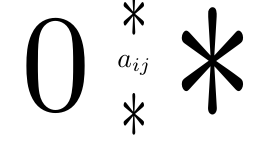
\begin{tikzpicture}[baseline={(current bounding box.center)}]
\node(NR1)[xscale=5,yscale=5]{$0$};
\node[right of = NR1](NR2){$a_{ij}$};
\node[right of = NR2,xscale=6,yscale=9](NR3){$*$};
\node[above of = NR2,yscale=3.5,xscale=2,yshift=-0.3em](NR16){$*$};
\node[below of = NR2,yscale=3.5,xscale=2,yshift=0.3em]{$*$};
\pgfresetboundingbox
\path[use as bounding box] ([xshift=2em,yshift=-2em]NR1.north west) rectangle ([yshift=3em,xshift=-2.5em]NR3.south east);
\node[above of = NR16](NR6){erste Spalte $\ne0$};
\node[above of = NR6,yshift=-1.5em]{$a_{ij\ne0}$};
\draw[->] ([yshift=0.5em]NR6.south) -- ([yshift=-1em]NR16.north);
\end{tikzpicture}
\right)\overset{Z_i\leftrightarrow Z_1}\sim
\left(
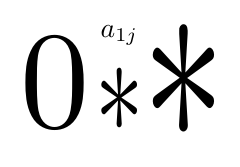
\begin{tikzpicture}[baseline={(current bounding box.center)}]
\node(NR1)[xscale=5,yscale=5]{$0$};
\node[above right of = NR1,xshift=3,yshift=-3](NR2){$a_{1j}$};
\node[below of = NR2,xscale=3.5,yscale=5,yshift=1](NR33){$*$};
\node[right of = NR1,xscale=6,yscale=9,xshift=3](NR4){$*$};
\pgfresetboundingbox
\path[use as bounding box] ([yshift=2em,xshift=-1em]NR1) rectangle ([yshift=-2em,xshift=1em]NR4);
\node[above of = NR2]{$a_{1j}\ne0$};
\end{tikzpicture}
\right)
\overset{Z_1\leftarrow\frac1{a_{1j}}Z_1}\sim
\left(
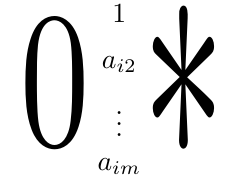
\begin{tikzpicture}[baseline={(current bounding box.center)}]
\node(NZ1)[xscale=5,yscale=7]{$0$};
\node[above right of = NZ1,xshift=3,yshift=0.5em](NZ2){$1$};
\node[below of = NZ2,yshift=1em](NZ33){$a_{i2}$};
\node[below of = NZ33,yshift=1em](NZ44){$\vdots$};
\node[below of = NZ44,yshift=1em](NZ55){$a_{im}$};
\node[right of = NZ1,xscale=6,yscale=12,xshift=3](NZ4){$*$};
\pgfresetboundingbox
\path[use as bounding box] ([yshift=2em,xshift=-1em]NZ1) rectangle ([yshift=-2.4em,xshift=1em]NZ4);
\end{tikzpicture}
\right)\\[1.2em]
\overset{Z_2\leftarrow Z_2-a_{i2}Z_1}{\overset{Z_3\leftarrow Z_3 - a_{i3}Z_1}{\underset{Z_m\leftarrow Z_m-a_{im}Z_1}{\underset\vdots\sim}}}
\left(
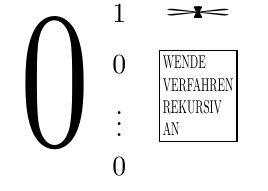
\begin{tikzpicture}[baseline={(current bounding box.center)}]
\node(NC1)[xscale=5,yscale=7]{$0$};
\node[above right of = NC1,xshift=3,yshift=0.5em](NC2){$1$};
\node[below of = NC2,yshift=1em](NC33){$0$};
\node[below of = NC33,yshift=1em](NC44){$\vdots$};
\node[below of = NC44,yshift=1em](NC55){$0$};
\node[right of = NC2,xscale=6](NC4){$*$};
\node[draw,align=left,below of = NC4,xscale=0.4,yscale=0.67,yshift=-0.2em] (NCU) {WENDE\\VERFAHREN\\REKURSIV\\AN};
\pgfresetboundingbox
\path[use as bounding box] ([yshift=2em,xshift=-1em]NC1) rectangle ([yshift=-2.4em,xshift=1.5em]NCU);
\end{tikzpicture}
\right)\sim\ldots\sim B
\end{multline*}
\end{algo}

\red{Bis hierher müssen wir am 2. Dezember kommen.}

\begin{algo}\label{5.2.4}
Eine Matrix $B\in K^{m\times n}$ in Stufenform kann man wie folgt in eine Matrix $C\in K^{m\times n}$ in reduzierter Stufenform überführen:
\begin{align*}
B&\overset{Z_i\leftarrow\frac1{b_{ij_i}}Z_i}{\underset{(i\in\{1,\ldots,r\})}\sim}
\begin{tikzpicture}[baseline=(current bounding box.center)]
  \matrix(A)[matrix of math nodes,left delimiter=(,right delimiter=),ampersand replacement=\&]
  {
    {}\&[3em]1\&[5em]b_{1j_2}\&[2em]b_{1j_3}\&[2em]\&[2em]b_{1j_r}\&[3em]\\
    \&\&1\&b_{2j_3}\&\&b_{2j_r}\\
    \&\&\&1\\
    \&\&\&\&\ddots\&b_{(r-1)j_r}\\
    \&\&\&\&\&1\\
    {}\\
    {}\\
    {}\\
    {}\\
  };
    \draw[loosely dotted,thick] (A-2-6.south) -- (A-4-6.north);
    \draw (A-1-2.north west) -- (A-1-2.south west) -|(A-2-3.south west) -|(A-3-4.south west) -|(A-4-5.north west);
    \draw (A-4-5.south east) -|(A-5-6.south west) -- (A-5-6.south east) -- ([shift={(4em,0)}]A-5-6.south east);
\node[anchor=south west,scale=5] at ([shift={(4em,-1em)}]A.south west) {0};
\node[anchor=north east,xscale=7,yscale=14] at ([shift={(2.5em,4em)}]A.north east) {*};
\node[anchor=west,xscale=13,yscale=7,xshift=0.15em] at ([shift={(-2em,-1em)}]A-2-3.east) {*};
\node[anchor=west,xscale=5,yscale=5] at ([shift={(-2em,-1.5em)}]A-1-3.east) {*};
\node[anchor=west,xscale=13,yscale=2] at ([shift={(-1em,0)}]A-1-1.east) {*};
\end{tikzpicture}\\[-7em]
&\overset{Z_i\leftarrow Z_i-b_{ij_rZ_r}}{\underset{(i\in\{1,\ldots,r-1\})}\sim}
\begin{tikzpicture}[baseline=(current bounding box.center)]
  \matrix(A)[matrix of math nodes,left delimiter=(,right delimiter=),ampersand replacement=\&]
  {
    {}\&[3em]1\&[5em]b_{1j_2}\&[2em]b_{1j_3}\&[2em]\&[2em]0\&[3em]\\
    \&\&1\&b_{2j_3}\&\&\\
    \&\&\&1\\
    \&\&\&\&\ddots\&0\\
    \&\&\&\&\&1\\
    {}\\
    {}\\
    {}\\
    {}\\
  };
    \draw[loosely dotted,thick] (A-1-6.south) -- (A-4-6.north);
    \draw (A-1-2.north west) -- (A-1-2.south west) -|(A-2-3.south west) -|(A-3-4.south west) -|(A-4-5.north west);
    \draw (A-4-5.south east) -|(A-5-6.south west) -- (A-5-6.south east) -- ([shift={(4em,0)}]A-5-6.south east);
\node[anchor=south west,scale=5] at ([shift={(4em,-1em)}]A.south west) {0};
\node[anchor=north east,xscale=7,yscale=14] at ([shift={(2.5em,4em)}]A.north east) {*};
\node[anchor=west,xscale=13,yscale=7,xshift=0.15em] at ([shift={(-2em,-1em)}]A-2-3.east) {*};
\node[anchor=west,xscale=5,yscale=5] at ([shift={(-2em,-1.5em)}]A-1-3.east) {*};
\node[anchor=west,xscale=13,yscale=2] at ([shift={(-1em,0)}]A-1-1.east) {*};
\end{tikzpicture}\\[-5em]
&\overset{Z_i\leftarrow Z_i-b_{ij_{r-1}Z_{r-1}}}{\underset{(i\in\{1,\ldots,r-2\})}\sim}\ldots\\[3em]
&\qquad\quad\ \vdots\\[-3em]
&\overset{Z_i\leftarrow Z_i-b_{ij_2Z_2}}{\underset{(i\in\{1,\ldots,1\})}\sim}
\begin{tikzpicture}[baseline=(current bounding box.center)]
  \matrix(A)[matrix of math nodes,left delimiter=(,right delimiter=),ampersand replacement=\&]
  {
    {}\&[3em]1\&[5em]0\&[2em]0\&[2em]\&[2em]0\&[3em]\\
    \&\&1\&0\&\&\\
    \&\&\&1\\
    \&\&\&\&\ddots\&0\\
    \&\&\&\&\&1\\
    {}\\
    {}\\
    {}\\
    {}\\
  };
    \draw[loosely dotted,thick] (A-1-6.south) -- (A-4-6.north);
    \draw (A-1-2.north west) -- (A-1-2.south west) -|(A-2-3.south west) -|(A-3-4.south west) -|(A-4-5.north west);
    \draw (A-4-5.south east) -|(A-5-6.south west) -- (A-5-6.south east) -- ([shift={(4em,0)}]A-5-6.south east);
\node[anchor=south west,scale=5] at ([shift={(4em,-1em)}]A.south west) {0};
\node[anchor=north east,xscale=7,yscale=14] at ([shift={(2.5em,4em)}]A.north east) {*};
\node[anchor=west,xscale=13,yscale=7] at ([shift={(-2em,-1em)}]A-2-3.east) {*};
\node[anchor=west,xscale=5,yscale=5] at ([shift={(-2em,-1.5em)}]A-1-3.east) {*};
\node[anchor=west,xscale=13,yscale=2] at ([shift={(-1em,0)}]A-1-1.east) {*};
\end{tikzpicture}=C
\end{align*}
\end{algo}

\begin{bem}\label{5.2.5}
Es ist nun geklärt, wie man homogene lineare Gleichungssysteme löst:
\begin{enumerate}[\normalfont(a)]
\item Bringe Koeffizientenmatrix auf Stufenform [$\to$ \ref{5.2.3}]
\item Bringe sie sogar in \emph{reduzierte} Stufenform [$\to$ \ref{5.2.4}]
\item Schreibe die Lösungsmenge als Spann [$\to$ \ref{5.1.13}]
\end{enumerate}
\end{bem}

\begin{bsp}\label{5.2.6}
$K = \F_5, n = 4$
$$ (*)\qquad
\begin{array}{l*{6}{l}}
\overline{4}x_2 & + x_3 & + \overline{3}x_4 & & = 0\\
\overline{2}x_1 & + \overline{3}x_2 & + x_4 & & = -\overline{2}x_3 \\
x_1 & + \overline{2}x_2 & +\overline{4}x_4 &+ \overline{3}x_3 &=0\\
\overline{2}x_1 & +\overline{4}x_2 & +x_3 & +\overline{3}x_4 & = 0
\end{array}
$$
kann man schreiben als
\[(*)\qquad Ax = 0\qquad (x\in {\F_5}^4)\] 
\begin{align*}
\text{mit }A:=\begin{pmatrix}
\overline{0} & \overline{4} & \overline{1} & \overline{3}\\
\overline{2} & \overline{3} & \overline{2} & \overline{1}\\
\overline{1} & \overline{2} & \overline{3} & \overline{4}\\
\overline{2} & \overline{4} & \overline{1} & \overline{3}
\end{pmatrix}&\overset{\over{Z_1\leftrightarrow Z_3}{\over{Z_2\leftarrow Z_2-2Z_1}{Z_4\leftarrow Z_4-\overline{2}Z_1}}}{\sim}\begin{pmatrix}
\overline{1} & \overline{2} & \overline{3} & \overline{4}\\
\overline{0} & \overline{4} & \overline{1} & \overline{3}\\
\overline{0} & \overline{4} & \overline{1} & \overline{3}\\
\overline{0} & \overline{0} & \overline{0} & \overline{0}
\end{pmatrix}\overset{Z_3\leftarrow Z_3-Z_2}{\sim}\begin{pmatrix}
\overline{1} & \overline{2} & \overline{3} & \overline{4}\\
\overline{0} & \overline{4} & \overline{1} & \overline{3}\\
\overline{0} & \overline{0} & \overline{0} & \overline{0}\\
\overline{0} & \overline{0} & \overline{0} & \overline{0}
\end{pmatrix}\\
&\overset{Z_2\leftarrow \frac{1}{\overline4}Z_2}{\sim}\begin{pmatrix}
\overline{1} & \overline{2} & \overline{3} & \overline{4}\\
\overline{0} & \overline{1} & \overline{4} & \overline{2}\\
\overline{0} & \overline{0} & \overline{0} & \overline{0}\\
\overline{0} & \overline{0} & \overline{0} & \overline{0}
\end{pmatrix}\overset{Z_1\leftarrow Z_1-2Z_2}{\sim}\begin{pmatrix}
\tikz[baseline=(m1.base)]\node(m1){$\overline{1}$}; & \overline{0} & \overline{0} & \overline{0}\\
\overline{0} & \tikz[baseline=(m2.base)]\node(m2){$\overline{1}$}; & \overline{4} & \tikz[baseline=(m3.base)]\node(m3){$\overline{2}$};\\
\overline{0} & \overline{0} & \overline{0} & \overline{0}\\
\overline{0} & \overline{0} & \overline{0} & \overline{0}
\end{pmatrix}
\begin{tikzpicture}[overlay]
\draw (m1.north west) -- (m1.south west) -- (m2.north west) -- (m2.south west) -- (m3.south east);
\end{tikzpicture}.
\end{align*}
reduzierte Stufenform\\
Stufenpositionen 1, 2\\
abhängig: $x_1, x_2$\\
frei: $x_3,x_4$

Die Lösungsmenge von $(*)$ ist
\begin{align*}
\Set{x\in {\F_5}^4 | Ax = 0}&=\Set{x\in {\F_5}^4 | x_1 = 0, x_2 = -\overline{4}x_3-\overline{2}x_4 = x_3+\overline{3}x_4} \\
&=\Set{\cvec{0\\x_3+3x_4\\x_3\\x_4} | x_3,x_4\in \F_5}\\
&=\Set{x_3\cvec{\overline{0}\\\overline{1}\\\overline{1}\\\overline{0}} +x_4\cvec{\overline{0}\\\overline{3}\\\overline{0}\\\overline{1}} | x_3, x_4\in \F_5}\\
&=\spann{\cvec{\overline{0}\\\overline{1}\\\overline{1}\\\overline{0}},\cvec{\overline{0}\\\overline{3}\\\overline{0}\\\overline{1}}}.
\end{align*}
\end{bsp}

\begin{bem}\label{5.2.7}
Ein homogenes lineares Gleichungssystem mit weniger Gleichungen als Unbekannten hat immer eine nichttriviale Lösung (eine Lösung $\neq 0$), denn mit \ref{5.2.3} und \ref{5.2.4} kann man seine Koeffizientenmatrix in reduzierter Stufenform annehmen und da diese Matrix breiter als hoch ist, hat das Gleichungssystem dann eine freie Unbekannte [$\to$ \ref{5.1.12}].
\end{bem}

\begin{bem}\label{5.2.8}
Beim Lösen von homogenen linearen Gleichungssystemen kann es manchmal sinnvoll sein, die Unbekannten $x_1,\ldots,x_n$ anders zu nummerieren, um schneller zu einer Koeffizientenmatrix in reduzierter Stufenform zu gelangen. Da man dies manchmal erst im Laufe der Berechnung bemerkt, kann man auch \emph{Spalten} vertauschen, wenn man sich merkt, welche Spalte zu welcher Unbekannten gehört.
\end{bem}

\begin{bsp}\label{5.2.9}
$Ax= 0\ (x\in\R^5)$ mit $A=\begin{pmatrix}
1 & 0 & 0 & 3 & 1\\
2 & 0 & 1 & 3 & 1\\
3 & 1 & 0 & 3 & 1
\end{pmatrix}$.
$$A\overset{Z_2\leftarrow Z_2-Z_1}{\underset{Z_3\leftarrow Z_3-Z_1}{\sim}}\begin{pmatrix}
1 & 0 & 0 & 3 & \tikz[baseline=(m1.base)]\node(m1){1};\\
1 & 0 & \tikz[baseline=(m2.base)]\node(m2){1}; & 0 & 0\\
\tikz[baseline=(m4.base)]\node(m4){2}; & \tikz[baseline=(m3.base)]\node(m3){1}; & 0 & 0 & 0
\end{pmatrix}$$
\begin{tikzpicture}[overlay]
\draw (m1.north east) -- (m1.south east) -- (m2.north east) -- (m2.south east) -- (m3.north east) -- (m3.south east) -- (m4.south west);
\end{tikzpicture}

\bigskip
$$\left[A\overset{\displaystyle\text{VORSICHT}\qquad}{\underset{\text{wahrscheinlich}}{\not\sim}}\right] \begin{pmatrix}
\tikz[baseline=(m1.base)]\node(m1){1}; & \tikz[baseline=(m2.base)]\node(m2){3}; & \tikz[baseline=(m3.base)]\node(m3){0};           & \tikz[baseline=(m4.base)]\node(m4){0}; & \tikz[baseline=(m5.base)]\node(m5){1};\\
0 & 0 & \tikz[baseline=(m6.base)]\node(m6){1}; & 0 & 1\\
0 & 0 & 0 & \tikz[baseline=(m7.base)]\node(m7){1}; & \tikz[baseline=(m8.base)]\node(m8){2};
\end{pmatrix}
\begin{tikzpicture}[overlay]
\draw (m1.north west) -- (m1.south west) -- (m6.north west) -- (m6.south west) -- (m7.north west) -- (m7.south west) -- (m8.south east);

\node[above = 0 of m1]{$x_5$};
\node[above = 0 of m2]{$x_4$};
\node[above = 0 of m3]{$x_3$};
\node[above = 0 of m4]{$x_2$};
\node[above = 0 of m5]{$x_1$};
\end{tikzpicture}$$
reduzierte Stufenform\\
3 Stufen\\
Stufenpositionen 1, 3, 4\\
abhängig: $x_5,x_3,x_2$\\
frei: $x_4,x_1$
$$\Set{x\in \R^5 | Ax=0}=\Set{\cvec{x_1\\-2x_1\\-1x_1\\x_4\\-x_1-3x_4} | x_1,x_4\in \R}=\spann{\cvec{1\\-2\\-1\\0\\-1},\cvec{0\\0\\0\\1\\-3}}$$
\end{bsp}

\red{Bis hierher sollten wir am 6. Dezember kommen.}

\section{Dualität}

\begin{df}\label{5.3.1}
Ist $A=\begin{pmatrix}
a_{11} & \ldots & a_{1n}\\
\vdots & & \vdots\\
a_{m1} & \ldots & a_{mn}
\end{pmatrix}\in K^{m\times n}$, so nennt man 
$$\underbrace{\row}_\text{"`row space"'} A:=\spann{\cvec{a_{11}\\\vdots\\a_{1n}},\ldots,\cvec{a_{m1}\\\vdots\\a_{mn}}}\subseteq K^n$$
den \emph{Zeilenraum}\index{Matrix@{\bf Matrix}!Zeilenraum ($\row$)} und $\ker A:=\Set{x\in K^n | \underbrace{Ax}_\text{[$\to$ \ref{5.1.9}]}=0}$ den \emph{Kern}\index{Matrix@{\bf Matrix}!Kern ($\ker$)} von $A$.
\end{df}

\begin{sat}\label{5.3.2}
Sind $A,B\in K^{m\times n}$ in reduzierter Stufenform mit $\ker A=\ker B$, so gilt $A=B$.
\end{sat}
\begin{proof}
Wir zeigen $\forall n\in \N_0:\forall m\in \N_0:\forall A,B\in K^{m\times n}$:
$$((A,B \text{ in reduzierter Stufenform }\et \ker A=\ker B)\Longrightarrow A=B)$$
durch Induktion nach $n$.
\begin{itemize}
\item[\underline{$n=0$}] Sind $m\in\N_0$ und $A,B\in K^{m\times 0}$, so gilt $A=()=B$.
\item[\underline{$n-1\to n\quad(n\in\N)$}] Seien $m\in \N_0$ und $A,B\in K^{m\times n}$ in reduzierter Stufenform mit $\ker A=\ker B$. Zu zeigen: $A=B$.
\begin{enumerate}[{Fall }1:]
\item
$A=\begin{pmatrix}0&&&\\\vdots&&

\begin{tikzpicture}[overlay]\node[xshift=-0.3em,yshift=0.5em,scale=5]{$*$};\end{tikzpicture}&\\
0&&&
\end{pmatrix}$.

Dann $\begin{pmatrix}1\\0\\\vdots\\0\end{pmatrix}\in \ker A=\ker B$ und daher
$B=\begin{pmatrix}
0&&&\\
\vdots&&

\begin{tikzpicture}[overlay]\node[xshift=-0.3em,yshift=0.5em,scale=5]{$*$};\end{tikzpicture}&\\
0&&&
\end{pmatrix}$.
Schreibe $A=\begin{pmatrix}0&&&\\\vdots&&
\begin{tikzpicture}[overlay]\node[yshift=0.5em,scale=2.5]{$A'$};\end{tikzpicture}&\\
0&&&
\end{pmatrix}$ und
$B=\begin{pmatrix}0&&&\\\vdots&&
\begin{tikzpicture}[overlay]\node[yshift=0.5em,scale=2.5]{$B'$};\end{tikzpicture}&\\
0&&&
\end{pmatrix}$ mit $A',B'\in K^{m\times(n-1)}$. Dann sind $A'$ und $B'$ in reduzierter Stufenform und es gilt 
\begin{multline*}
\ker A'=\Set{\cvec{x_2\\\vdots\\x_n}\in K^{n-1} | \cvec{0\\x_2\\\vdots\\x_n}\in \ker A}\\
\overset{\ker A=\ker B}=\Set{\cvec{x_2\\\vdots\\x_n}\in K^{n-1} | \cvec{0\\x_2\\\vdots\\x_n}\in \ker B}=\ker B'
\end{multline*} und daher $A'=B'$ nach IV. Also $A=B$.






\item $A=\begin{pmatrix}1&&&&\\0&&&&\\
\vdots&&&

\begin{tikzpicture}[overlay]\node[xshift=-0.5em,yshift=1em,xscale=6,yscale=8]{$*$};\end{tikzpicture}&\\
0&&&&
\end{pmatrix}$


Dann $\cvec{1\\0\\\vdots\\0}\notin \ker A=\ker B$ und daher
$B=\begin{pmatrix}1&&&&\\0&&&&\\
\vdots&&&

\begin{tikzpicture}[overlay]\node[xshift=-0.5em,yshift=1em,xscale=6,yscale=8]{$*$};\end{tikzpicture}&\\
0&&&&
\end{pmatrix}$.





Schreibe $A=\begin{pmatrix}1&&\begin{tikzpicture}[overlay]\node[xshift=0.2em,yshift=0.25em,xscale=8,yscale=2]{$*$};\end{tikzpicture}&&\\
0&&&&\\
\vdots&&
\begin{tikzpicture}[overlay]\node[yshift=0.5em,xscale=2.5,yscale=4]{$A'$};\end{tikzpicture}&&\\
0&&&&
\end{pmatrix}$ und
$B=\begin{pmatrix}1&&\begin{tikzpicture}[overlay]\node[xshift=0.2em,yshift=0.25em,xscale=8,yscale=2]{$*$};\end{tikzpicture}&&\\
0&&&&\\
\vdots&&

\begin{tikzpicture}[overlay]\node[yshift=0.5em,xscale=2.5,yscale=4]{$B'$};\end{tikzpicture}&&\\
0&&&&
\end{pmatrix}$ mit $A',B'\in K^{(m-1)\times (n-1)}$. Dann sind $A'$ und $B'$ in reduzierter Stufenfom und es gilt
\begin{align*}
\ker A' &= \Set{\cvec{x_2\\\vdots\\x_n}\in K^{n-1} | \exists x_1\in K:\cvec{x_1\\\vdots\\x_n}\in \ker  A}\\
&=\Set{\cvec{x_2\\\vdots\\x_n}\in K^{n-1} | \exists x_1\in K:\cvec{x_1\\\vdots\\x_n}\in \ker B} = \ker B'
\end{align*}
und daher $A'=B'$ nach IV. Es bleibt nur noch zu zeigen, dass die jeweils ersten Zeilen von $A$ und $B$ übereinstimmen.
\begin{itemize}
\item[\emph{Behauptung 1:}] $A$ und $B$ haben dieselben Stufenpositionen.
\item[\emph{Begründung:}] 1 ist Stufenposition von $A$ und von $B$. Sei $j\in \left\{2,\ldots, n\right\}$. Dann $j$ Stufenposition von $A\iff j-1$ Stufenposition von $A' = B'\iff j$ Stufenposition von $B$.
\item[\emph{Behauptung 2:}] Die Gleichungssysteme $Ax = 0$ und $Bx = 0$ $(x\in K^n)$ haben dieselben abhängigen und freien Unbekannten.
\item[\emph{Begründung:}] folgt sofort aus Behauptung 1.
\end{itemize}
Sei nun $j\in \left\{2,\ldots,n\right\}$, $a$ der $j$-te Eintrag von $A$ und $b$ der $j$-te Eintrag von $B$ in der ersten Zeile. Zu zeigen: $a = b$. Ist $j$ eine Stufenposition von $A$, so nach Behauptung 1 auch von $B$ und daher $a = 0 = b$.
Sei also nun $j$ keine Stufenposition von $A$. Dann ist $x_j$ frei (für beide Gleichungssysteme, siehe Behauptung 2) und man findet $x\in \ker A = \ker B$ mit $x_j = 1$ und $x_k = 0$ für alle anderen freien Unbekannten $x_k$. Es folgt $1\cdot x_1 + a x_j = 0 = 1\cdot x_1+ bx_j$ und damit $a = -x_1 = b$.\qedhere
\end{enumerate}
\end{itemize}
\end{proof}

\begin{bem}\label{5.3.3}
Ist $A\in K^{m\times n}$, so
$$\ker A = \left\{x\in K^n\mid \forall a\in \row A: a_1x_1+\dots+a_nx_n = 0\right\}\text{ [$\to$ \ref{5.1.9}, \ref{5.3.1}].}$$
\end{bem}

\begin{sat}\label{5.3.4}
Seien $A,B\in K^{m\times n}$. Dann
$$A\sim B \iff \ker A = \ker B\iff \row A = \row B$$
\end{sat}
\begin{proof}
Zeilenoperationen auf einer Matrix aus $K^{m\times n}$ ändern weder ihre Äquivalenzklasse [$\to$ \ref{5.2.2}], noch ihren Kern [$\to$ \ref{5.1.14} (b)] noch ihren Zeilenraum (sieht man leicht). Also können wir nach \ref{5.2.3} und \ref{5.2.4} $A$ und $B$ in reduzierter Stufenform annehmen. Dann
$$\ker A = \ker B \overset{\text{\ref{5.3.2}}}{\Longrightarrow} A = B \Longrightarrow A \sim B \Longrightarrow \row A = \row B \overset{\text{\ref{5.3.3}}}{\Longrightarrow} \ker A = \ker B.$$
\end{proof}

\begin{kor}\mbox{}\label{5.3.5}
{\rm[$\to$ \ref{5.3.3}]} Ist $A\in K^{m\times n}$, so
$$\row A = \left\{a\in K^n \mid\forall x\in \ker A: a_1x_1+\ldots+a_nx_n = 0\right\}.$$
\end{kor}
\begin{proof}
Sei $A\in K^{m\times n}$.
\begin{itemize}
\item["`$\subseteq$"'] ist klar nach Def. \ref{5.3.1}.
\item["`$\supseteq$"'] Sei $a\in K^n$ mit $\forall x\in \ker A:a_1x_1+\ldots+a_nx_n = 0$.\\
Dann $\ker A=\ker\begin{pmatrix}&&\\
&
\begin{tikzpicture}[overlay]\node[xshift=0.2em,yshift=0.25em,xscale=6,yscale=4]{$A$};\end{tikzpicture}&\\
&&\\
a_1&\ldots&a_n\end{pmatrix}
= \ker\begin{pmatrix}&&\\
&
\begin{tikzpicture}[overlay]\node[xshift=0.2em,yshift=0.25em,xscale=6,yscale=4]{$A$};\end{tikzpicture}&\\
&&\\
0&\ldots&0\end{pmatrix}$ und daher 
$$\cvec{a_1\\\vdots\\a_n}\in\row
\begin{pmatrix}&&\\
&
\begin{tikzpicture}[overlay]\node[xshift=0.2em,yshift=0.25em,xscale=6,yscale=4]{$A$};\end{tikzpicture}&\\
&&\\
a_1&\ldots&a_n\end{pmatrix}
\overset{\text{\ref{5.3.4}}}{=}\row
\begin{pmatrix}&&\\
&
\begin{tikzpicture}[overlay]\node[xshift=0.2em,yshift=0.25em,xscale=6,yscale=4]{$A$};\end{tikzpicture}&\\
&&\\
0&\ldots&0\end{pmatrix}=\row A.$$
\end{itemize}
\end{proof}

\begin{kor}\mbox{}\label{kerrow}
Ist $A\in K^{m\times n}$ und $X\in K^{\ell\times n}$, so
\[\ker A=\row X\iff\ker X=\row A.\]
\end{kor}

\begin{proof}
Aus Symmetriegründen reicht es "`$\implies$"' zu zeigen. Gelte also $\ker A=\row X$.
Aus $\ker A\supseteq\row X$ folgt leicht $\ker X\supseteq\row A$. Es bleibt $\ker X\subseteq\row A$ zu zeigen.
Sei hierzu $a\in\ker X$. Zu zeigen ist $a\in\row A$. Nach Korollar \ref{5.3.5} reicht es hierzu zu zeigen, dass
\[a_1x_1+\ldots+a_nx_n=0\]
für alle $x\in\ker A$. Diese Gleichung ist für alle Zeilen $x$ von $X$ klar wegen $a\in\ker X$ und der
Kommutativität der Multiplikation in $K$. Damit ist sie aber
auch klar für alle $x$ aus dem Zeilenraum $\row X$ von $X$. Dieser ist aber nach Voraussetzung gleich $\ker A$.
\end{proof}

\begin{bem}\label{dualproblem}
Gegeben seien $x^{(1)},\ldots,x^{(\ell)}\in K^n$. Wir wollen ein homogenes lineares Gleichungssystem ohne redundante Gleichungen finden, dessen Lösungsmenge genau
$\spann{x^{(1)},\ldots,x^{(\ell)}}$ ist. Diese sogenannte \emph{duale Aufgabe} kann man wegen \ref{kerrow} wie folgt lösen:

Schreibe $x^{(1)},\ldots,x^{(\ell)}$ als Zeilen der Matrix $X\in K^{\ell\times n}$. Löse das Gleichungssystem
\[X\cdot a = 0\qquad(a\in K^n)\]
und fasse die gefundenen Basislösungen $a^{(1)},\ldots, a^{(m)}\in K^n$ als Zeilen einer Matrix $A\in K^{m\times n}$ auf. Es ist dann
\[A\cdot x = 0\qquad(x\in K^n)\]
ein Gleichungssystem wie gewünscht.
\end{bem}

\begin{bsp}\label{dualex}
Wir suchen ein Gleichungssystem, dessen Lösungsmenge
$\spann{\cvec{2\\1\\0},\cvec{0\\1\\1}}$ ist.
\begin{align*}
X:= \begin{pmatrix}
2 & 1 & 0\\
0 & 1 & 1
\end{pmatrix}\overset{Z_1 \leftarrow \frac{1}{2}Z_1}{\sim}\begin{pmatrix}
1 & \frac{1}{2} & 0\\
0 & 1 & 1
\end{pmatrix}\overset{Z_1\leftarrow Z_1-\frac{1}{2}Z_2}{\sim}\begin{pmatrix}
\tikz[baseline=(m1.base)]\node(m1){$1$}; & 0 & -\frac{1}{2}\\
0 & \tikz[baseline=(m2.base)]\node(m2){$1$}; & \tikz[baseline=(m3.base)]\node(m3){$1$};
\end{pmatrix}
\begin{tikzpicture}[overlay]
\draw (m1.north west) -- (m1.south west) -- (m2.north west) -- (m2.south west) -- (m3.south east);
\end{tikzpicture}
\end{align*}
\begin{align*}
\Set{a\in \R^3 | X\cdot a = 0} &= \Set{a\in\R^3 | a_1 = \frac{1}{2}a_3, a_2 = -a_3}= \Set{\cvec{\frac{1}{2}a_3\\-a_3\\a_3}| a_3\in\R}\\
&= \spann{\cvec{\frac{1}{2}\\-1\\1}}= \spann{\cvec{1\\-2\\2}}
\end{align*}
$x_1-2x_2+2x_3 = 0$ $(x\in\R^3)$ ist ein Gleichungssystem wie gesucht.
\end{bsp}
\end{document}